\section{Game Design}

\todo{maybe reiterate/summarize research goals? a game that encourages
  collaborative dialog in order to solve a task in a virtual
  environment; interested in situated language use, so dialog about
  the environment; environment should be simple enough that can be
  modeled using an automated planner}

In this two-player game, each player is situated in a maze created
from obstacles and traps of various kinds.  Figure
\ref{fig:player-screenshots} illustrates what the game interface may
look like for each player at some point in the
game\footnote{While the game is fully playable, the interface is still
  a prototype in which everything is represented by differently
  colored blocks.}. The red block is player one's avatar, the green
block player two's avatar. The purple block is the ball, which needs
to be pushed to the goal represented by the orange block. The white
and gray blocks are portals. Portals come in pairs -- if the ball or
player enter one portal, they exit through another one --- and connect
different areas of one player's environment or link one player's
environment with the other's. The white portals are open to both the
ball and the player; the gray portals can only be used by the ball.

%% Commented this out because we already say something similar in the
%% previous section. KS
%% The goal for this game was to have two players communicate and
%% collaborate with each other in order to push a block to a certain
%% location on the screen, the goal. The game consists of two different
%% screens of the same size: one that is only visible to player one and
%% another that is only visible to player two. Figure
%% \ref{fig:player-screenshots} shows an example screen for player one
%% and two.

\begin{figure}
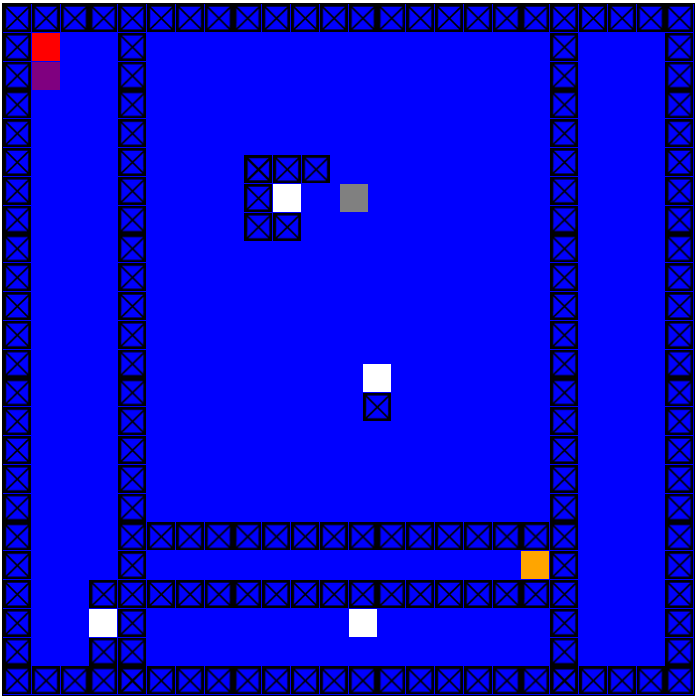
\includegraphics[scale=0.27]{playerview1.png} 
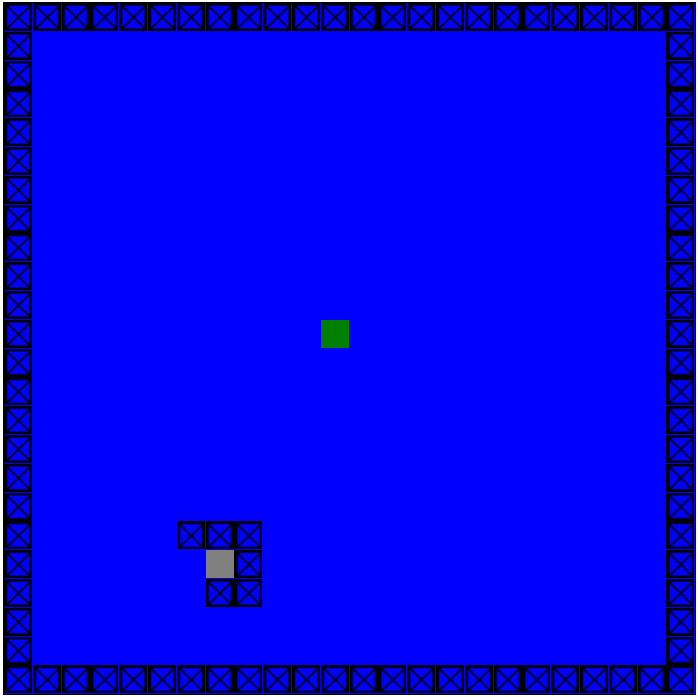
\includegraphics[scale=0.27]{playerview2.png}
\caption{Sample game screens for players one and two.\todo{let's get
    screenshots that show the chat area; I will try to fix css today
    or tomorrow - KS}}
\label{fig:player-screenshots}
\end{figure}

% what players do; moving the ball

The players can move their avatars using the arrow keys on their
keyboard. When they push the ball, it starts moving in the direction
of the push and only stops when it collides with an obstacle. If the
ball cannot move in the direction of the push (e.g. because there is
an obstacle), it (randomly) picks a direction that is free of
obstacles to move to, as illustrated in Figure
\ref{fig:pushing-against-wall}. This behavior makes sure that the ball
does not get trapped too easily.

\begin{figure}
\todo{Add images.}
\caption{Behavior of the ball.}
\label{fig:pushing-against-wall}
\end{figure}

% placing of blocks

Pressing the \todo{which?} key allows players to place an obstacle
into their partner's environment at the position that corresponds to
the player's current location. Each player can only place three blocks
on their partner's screen at a time. When the fourth block is placed,
the block that was placed first is deleted, as shown in Figure
\ref{fig:dropping-blocks}.

\begin{figure}
\hspace*{\fill}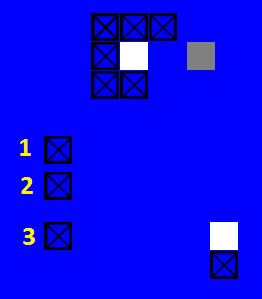
\includegraphics[width=0.45\columnwidth]{blocksplaced1-cropped.png}
\hspace*{\fill}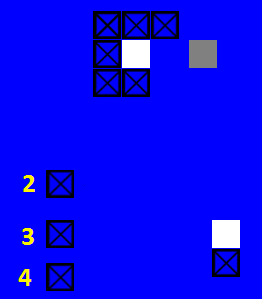
\includegraphics[width=0.45\columnwidth]{blocksplaced2-cropped.png}\hspace*{\fill}
\caption{Each player can place at most three obstacles at a time. When
  the fourth obstacle gets placed, the first one disappears.}
\label{fig:dropping-blocks}
\end{figure}

The players cannot place obstacles into their own environments, and
since obstacles are the only way to stop a ball that is moving, they
have to collaborate to control the balls movements. 


% chatting 

The environments are designed to force the players to work together
and communicate with each other.  The players can use a chat area next
to their game environment to coordinate their strategy and to give
instructions on where obstacles need to be placed.


% visibility of screens

We are creating three modes of the game by manipulating whether the
players can see their partner's environment, in order to study the
effect that additional shared information about the context has on
communication.  In the first mode, the players don't see their
partner's environment (as in Figure \ref{fig:player-screenshots}), but
the location of obstacles that get dropped into their environment give
them some hints where their partner is. In mode two, the players can
see a shadow of their partner's avatar moving around their own
environment, so that they always know where their partner is, but they
don't have any information about the layout of their partner's
environment. And in the third mode, the players see their
own environment and their partner's side by side.


% kinds of obstacles 

The game starts out with relatively simple environments, but gets more
complicated as additional kinds of obstacles and traps and more
complex variations of the task get introduced.  For example, there may
be pits which can swallow the ball (or player), bouncy obstacles which
reflect the ball when it hits them, moving fireballs which burn and
kill the ball or player, destructable barriers which the partner can
explode by dropping an obstacle onto them, or forking portals which
send the ball/player randomly to one of two exits (but which become
deterministic if the partner blocks one exit by dropping an obstacle
onto it). \todo{Is this too much to say? spoilers?}  At some level
each player is given their own set of one or more balls. This will
allow for some interesting variations on the task. For example, there
may be multiple goal positions and the players have to navigate their
balls to corresponding goals. Or the balls are numbered (e.g. player
one has balls number 1, 3 and 4 and player two has balls 2 and 5) and
the balls have to be push into goals in order. Or the balls have
colors and both players have to move a ball of the same color to a
goal before they can work on the next ball with a different color.
